\section{Experimental Setup}
\subsection{Radioactive Source: $^{152}\mathrm{Eu}$}
Europium-152 ($^{152}\mathrm{Eu}_{63}$) is a radioactive isotope of europium with a half-life of approximately 13.5 years. It decays primarily by electron capture and beta-plus emission to excited nuclear state of Samarium-152 ($^{152}\mathrm{Sm}_{62}$) and a small fraction of  Gadolinium-152 ($^{152}\mathrm{Gd}_{64}$)  through beta-minus decay. The subsequent de-excitation and decays of the daughter species leads to several gamma radiations, producing a range of characteristic gamma-ray lines.

\begin{figure}[h]
    \centering
    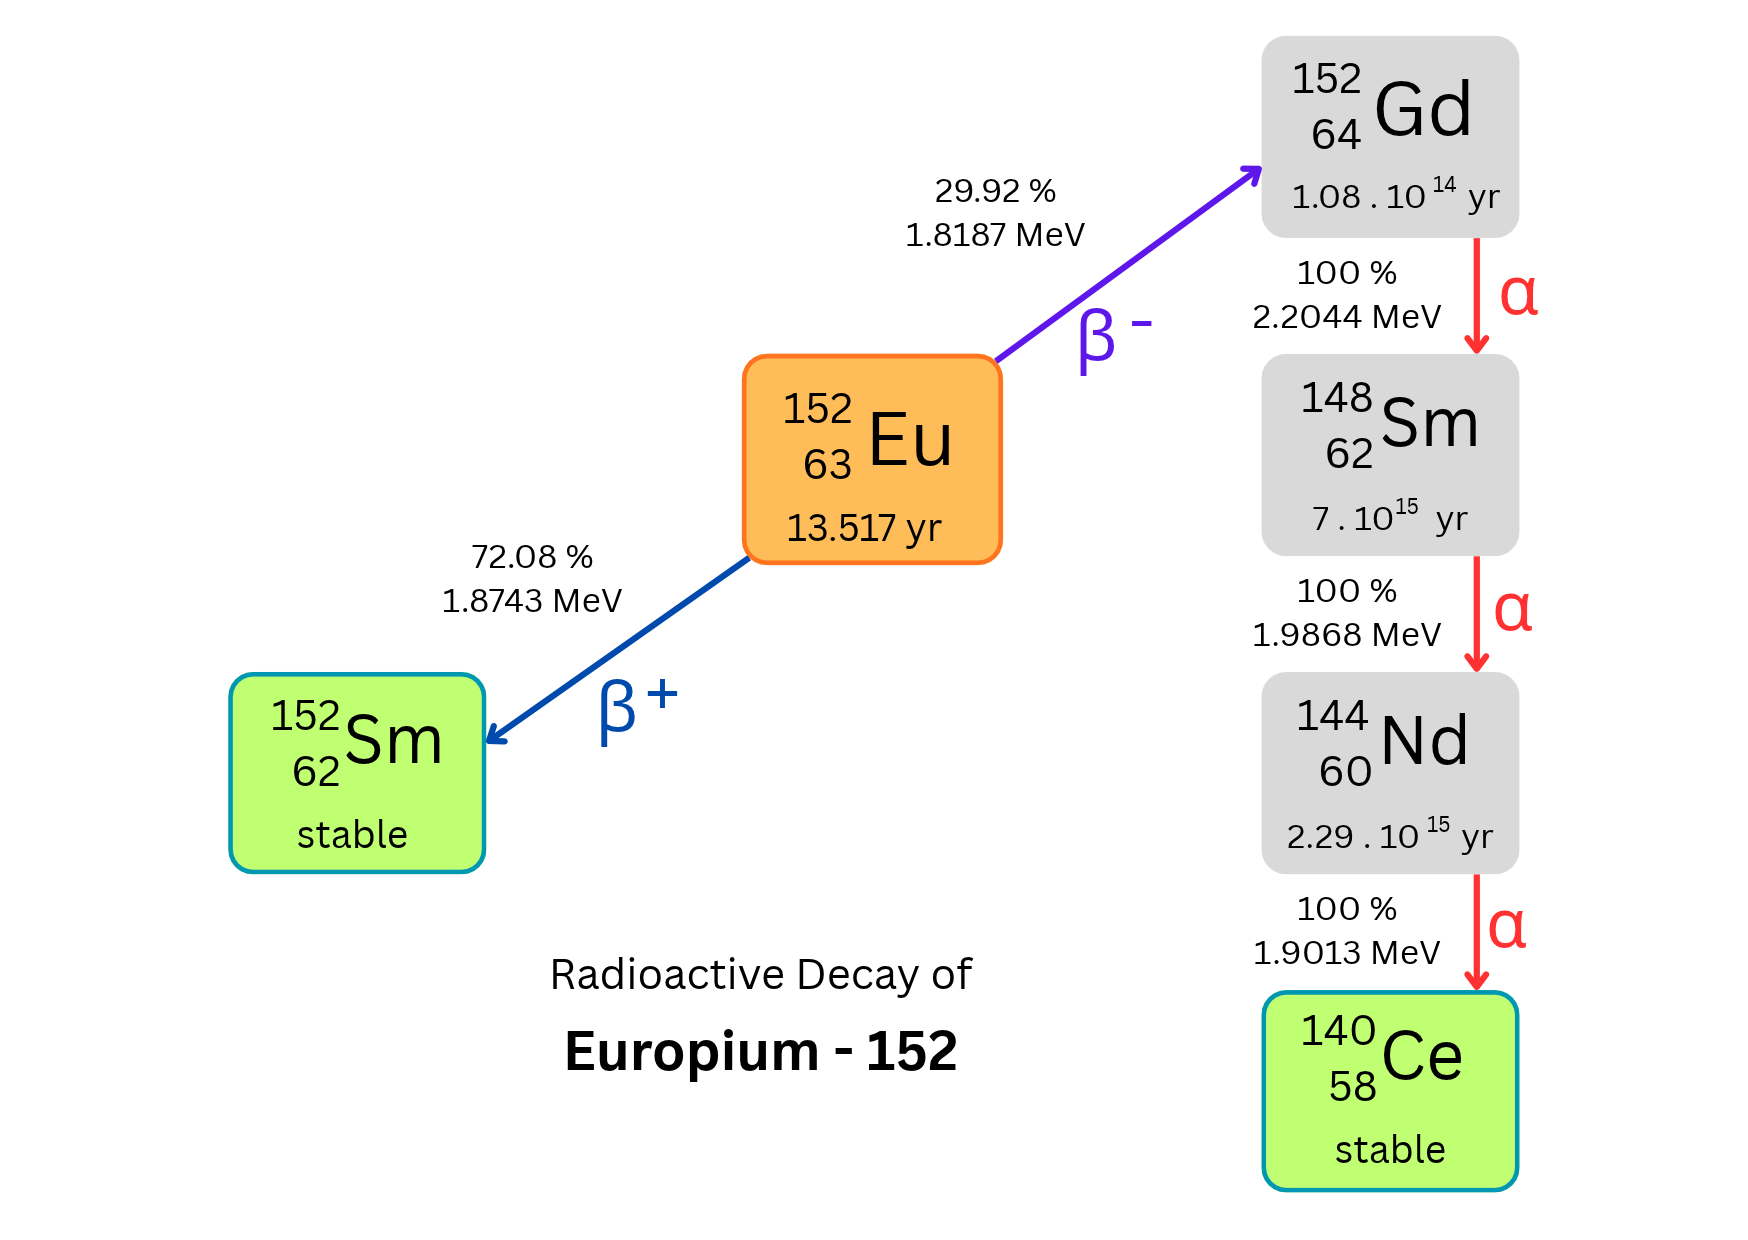
\includegraphics[width=0.7\linewidth]{Images/Eu.png}
    \caption{Europium 152 decay chain.}
    \label{Eu152 Decay}
\end{figure}

The decay of $^{152}\mathrm{Eu}$ produces a complex gamma-ray spectrum consisting of several discrete emission lines. Consequently, the source provides a set of well-characterized gamma-ray energies that can be used as reference values in spectroscopic measurements. Eu-152 is typically produced artificially in nuclear reactors through neutron activation of europium-151  \cite{Eu152, Jaeck_undated_Eu152}.

\subsection{Gamma-ray detector: $\mathrm{LaBr}_3\mathrm{(Ce)}$}
The basic elements of a scintillation detector are shown in the schematic below in Fig. \ref{scintillation_sch}. It consists of a scintillating material which is optically coupled to a photomultiplier either directly or via a light guide. As the radiation passes through the scintillator, exciting the atoms and molecules of the material causing light to be emitted, which is detected by the photomultiplier (PMT) tube. 

\begin{figure}[h]
    \centering
    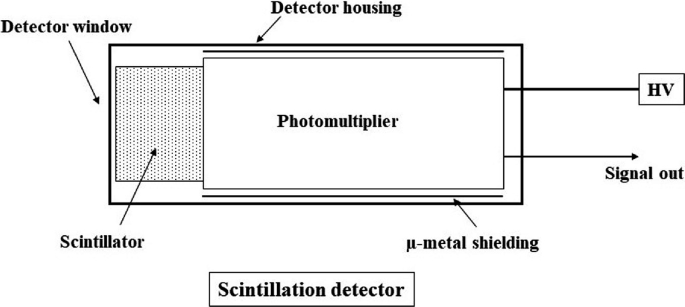
\includegraphics[width=0.7\linewidth]{Images/scintillation_dect_sch.png}
    \caption{Schematic diagram of a scintillation counter.}
    \label{scintillation_sch}
\end{figure}

Scintillator materials exhibit the property of \textit{luminescence}. Luminescent materials, absorb radiations and re-emit the energy in the form of visible light. If the reemission occurs within $10^{-8}$s (time taken for  atomic transitions), the process is usually called \textit{fluorescence}. However, if the reemission is delayed because of metastable excited state, the process is called \textit{phosphorescence} or \textit{afterglow}. In such cases the delay time between absorption and reemission may last anywhere from a few microseconds to hours depending on the material \cite{leo_scintillation}.

The time evolution of the reemission process in the material is described through a complicated two-component exponential decay as

\begin{equation}
    N = A \exp(\frac{-t}{\tau_f}) + B \exp(\frac{-t}{\tau_s})
\end{equation}

Where $\tau_f$ and $\tau_s$ are decay constants. For most scintillators, one component is generally much faster than the other referring the constants as \textit{fast} and \textit{slow} components. The relative magnitudes, $A$ and $B$, vary from material to material, although the fast components generally dominate. 

While many scintillating materials exist, not all are suitable as detector. In general a good scintillator should satisfy the following requirements:

\begin{enumerate}
    \item high efficiency for conversion of excited energy to fluorescent radiation
    \item transparency to its fluorescent radiation to allow transmission of light
    \item emission in a spectral range consistent with the spectral response of the PMTs
    \item a short decay constant, $\tau$
\end{enumerate}

Cerium-doped Lanthanum(III) bromide ($\mathrm{LaBr}_3\mathrm{(Ce)}$) is an inorganic scintillation detector, consisting of halide salt crystals of lanthanum with cerium ion impurities. Inorganic crystals have a higher number density and higher atomic number leading to greater stopping power, making it advantageous over organic and plastic scintillator. They also have some of the highest light outputs, resulting in better energy resolution. 

The gamma rays from the source interacts with the scintillating material through the photoelectric effect, Compton scattering and pair production. These interactions transfer energy to energetic electrons, which subsequently produce excitation and ionization within the scintillator. The deposited energy is converted into electronic excitation, which transfer the energy to luminescence centers, subsequently emitting optical photons. For $\mathrm{LaBr}_3\mathrm{(Ce)}$, the $\mathrm{Ce}^{3+}$ ions act as the activator centers responsible for efficient scintillation. The scintillation light output is approximately proportional to the energy deposited in the crystal.

\begin{figure}[h]
    \centering
    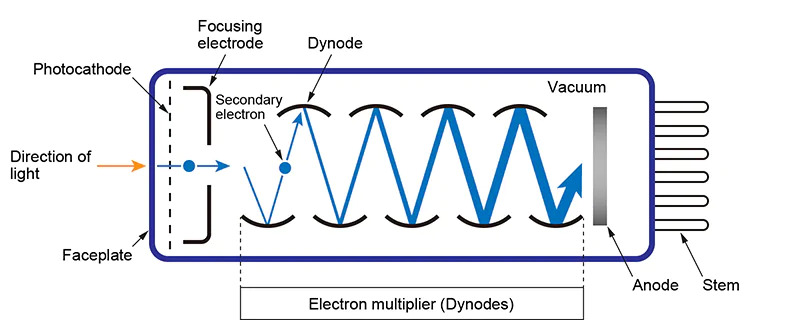
\includegraphics[width=0.6\linewidth]{Images/pmts.jpg}
    \caption{Schematic diagram of a photomultiplier tubes.}
    \label{pmts_sch}
\end{figure}

The photomultiplier tube (PMT), is a photoemissive device in which the absorption of a photon results in the emission of an electron. These detectors work by amplifying the electrons generated by a photocathode exposed to a photon flux. The schematic of a PMT is shown in Fig ~\ref{pmts_sch}. Photomultipliers acquire light through a glass or quartz window that covers a photosensitive surface, called a photocathode, which then releases electrons that are multiplied by electrodes known as metal channel dynodes. At the end of the dynode chain is an anode or collection electrode. Over a very large range, the current flowing from the anode to ground is directly proportional to the photoelectron flux generated by the photocathode \cite{PMT}.

The emitted optical photons from the scintillator are detected by a photomultiplier tube (PMT). The photocathode converts the photons into photoelectrons, which are multiplied through a series of dynodes before being collected at the anode. This produces an electrical pulse whose amplitude or integrated charge is related to the energy deposited in the scintillator. 

\subsection{Data Acquisition System: CAEN V1730}
The electrical signal pulse generated at the PMT anode is subsequently processed by the data acquisition system (DAQ). The DAQ system acquires the analog signals, and convert them into digital data and storing them for further analysis. In the present experiment, a \texttt{CAEN V1730} waveform digitizer is employed for this purpose.

\begin{figure}[t]
    \centering
    
\includegraphics[width=0.8\linewidth]{Images/DAQ_sch.png}
    \caption{Primary components of a data acquisition system.}
    \label{daq_sch}
\end{figure}

A waveform digitizer samples the input voltage signal at regular intervals, converting each sample into a digital value using an analog-to-digital converter (ADC). The digitizer waveform contains information about the temporal evolution of the detector pulse. Parameters such as pulse amplitude and integrated charge can subsequently be extracted and used to estimate the energy deposited in the detector. For a sampling frequency of $f_s$, the time interval between consecutive samples is 

\begin{equation*}
    \Delta t = \frac{1}{f_s}
\end{equation*}

A higher sampling frequency provides better temporal resolution and allows the digitizer to record rapidly varying detector pulses.

Each sampled voltage is converted into a digital value by the ADC. The resolution of the ADC, expressed in bits, determines the number of discrete digital levels available to represent the input voltage. For an $N$-bit ADC, the number of possible digital levels is
\begin{equation*}
    N_{\mathrm{levels}}=2^N
\end{equation*}

Thus, a 14-bit ADC can represent the input signal using \(2^{14}=16384\) discrete levels. The resulting sequence of digital samples represents the acquired detector waveform, which can be stored and processed for further analysis.

The \texttt{CAEN V1730} waveform digitizer used is a high-speed, multichannel digitizer designed for applications involving fast detector signals, including scintillation detectors coupled to PMTs. 

The \texttt{V1730} incorporates a 14-bit Flash ADC operating at a sampling frequency of $500$ MS/s (mega-samples per second). This corresponds to a sampling interval of 

\begin{equation*}
    \Delta t = \frac{1}{500\times10^6} = 2 \, \mathrm{ns}
\end{equation*}

The 14-bit resolution provides 16384 discrete digital levels for representing the input voltage. The digitizer also provides selectable input voltage ranges of $0.5$ Vpp and $2$ Vpp, allowing the acquisition range to be adjusted according to the amplitude of the incoming detector signals \cite{CAEN_daq}.

\begin{figure}[h]
    \centering
    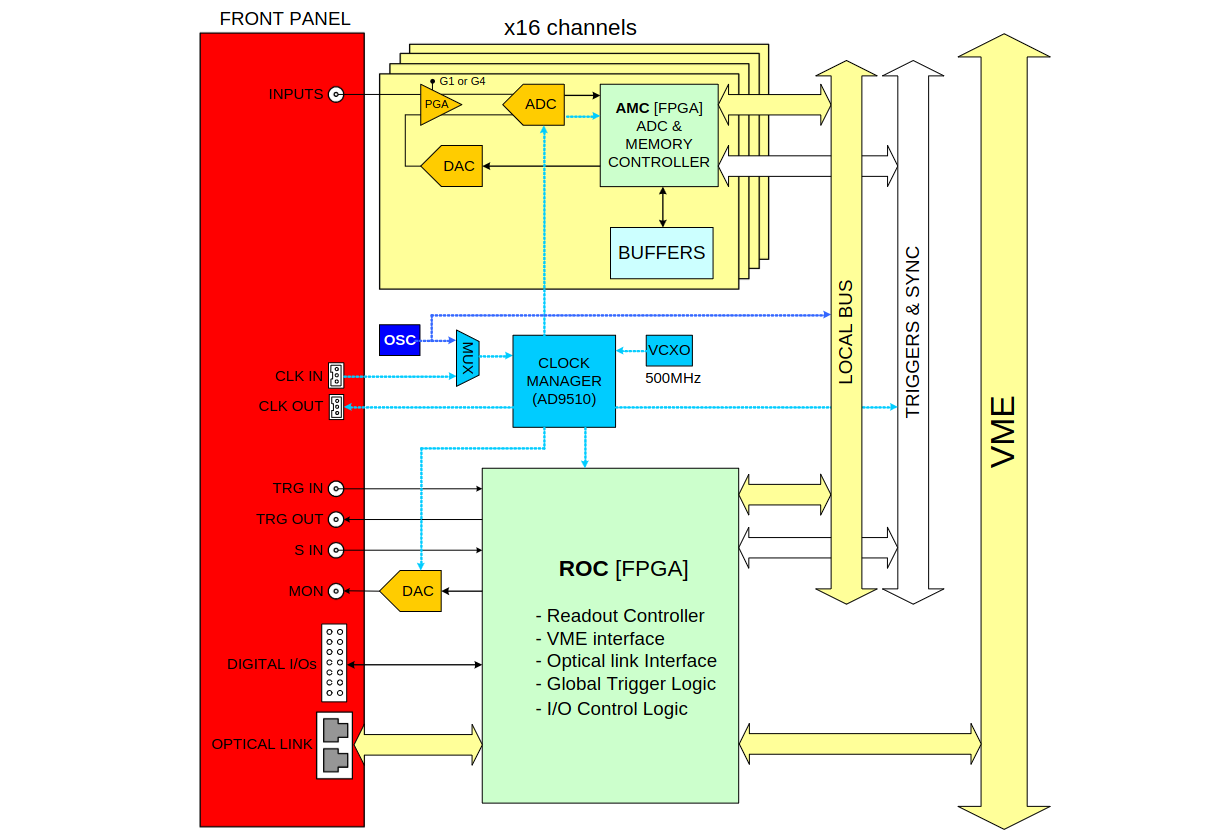
\includegraphics[width=0.7\linewidth]{Images/V1730_sc.png}
    \caption{Schematic of the CAEN V1730 DAQ system.}
    \label{caen_sch}
\end{figure}

% \begin{figure}[h]
%     \centering
%     \includegraphics[width=0.8\linewidth]{Images/V1730.png}
%     \caption{Schematic of the CAEN V1730 DAQ system.}
%     \label{caen_sch}
% \end{figure}

\subsection{Set-up schematic}

In the present experiment, the \texttt{CAEN V1730} is used to acquire the electrical pulses generated by the $\mathrm{LaBr}_3\mathrm{(Ce)}$ scintillation detector. The analog signals produced by the detector are supplied to the digitizer, where they are sampled and converted into digital waveforms. The acquired signals can subsequently be analyzed to extract pulse characteristics related to the energy deposited in the scintillator. By associating the extracted pulse information with the known gamma-ray energies emitted by the $^{152}\mathrm{Eu}$ source, the detector response can be characterized, and its energy calibration can be established.

\begin{figure}[h]
    \centering
    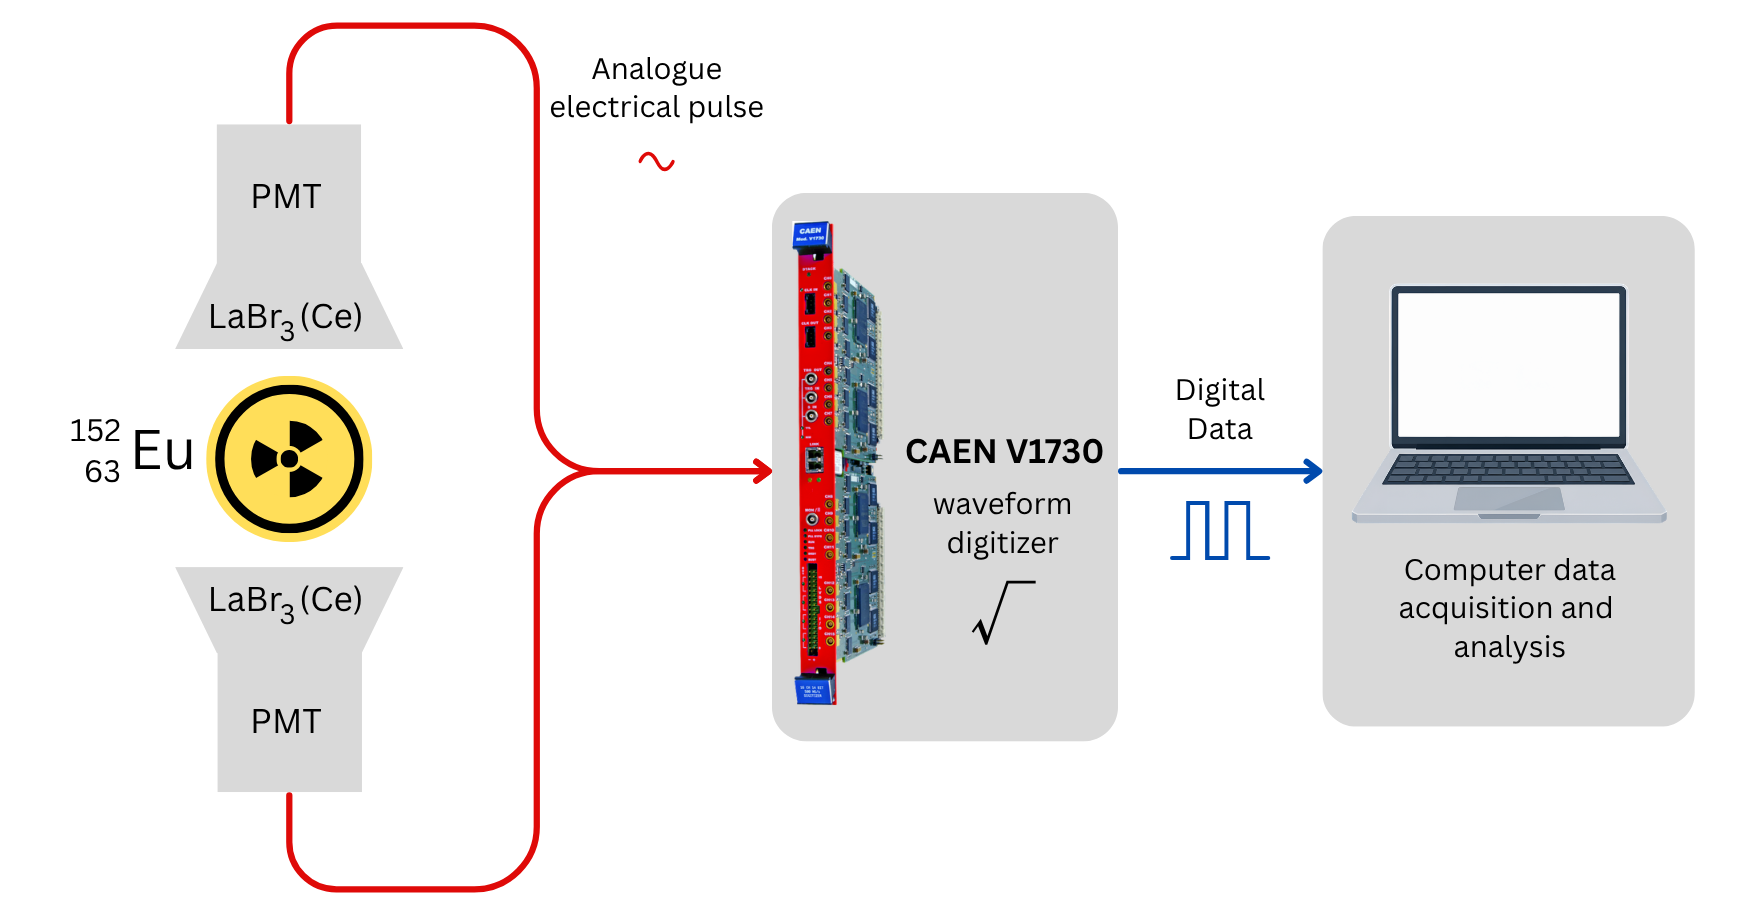
\includegraphics[width=0.8\linewidth]{Images/setup.png}
    \caption{Schematic of the Experimental Setup.}
    \label{expt_sch}
\end{figure}
